\section{Implementation}
\label{sec:implementation}
\emph{Watt's Happening} is implemented on Android OS version 4.0, API level $>$ 14. 
The Android OS provides a variety of APIs allowing access to application and hardware information.
Information that is not exposed via the API is obtained directly from the underlying operating system.

\subsection*{Logging}
When obtaining information, it is important to ensure \emph{Watt's Happening} remains relatively low-impact.
This is accomplished by using a time-based polling method of collecting data, as opposed to constant and intrusive observation.
Resource usage is obtained via the Managers provided in the Android API.
Battery level, GPS state, WiFi state, Bluetooth state, network connection and screen state are all collected and stored.
Application information including UID, name, network information transmitted and received, cpu usage, and runtime is collected and stored. 
While the majority of the application information is obtained from the Managers described above, cpu usage is not exposed via the API.
\emph{Watt's Happening} obtains cpu usage in the same manner as `top', `ps', and other standard system tools.
\emph{Watt's Happening} parses the data in the `proc' folder for each application.
Based on our iterative experimentation, information is polled every five minutes.
We believe this maintains the delicate balance between fine-grained information capture and battery used by \emph{Watt's Happening}.
There are some low duration, high-power events, such as BlueTooth pairing and GPS-based updates, that may not be captured by time-based polling.
To handle these cases, our framework allows for event listeners.
These events are logged when they occur. 

\subsection*{Analysis}
Although data is collected every five minutes, analysis is delayed until there is sufficient information to justify the overhead of performing the analysis.
The analysis performs two distinct tasks, aggregating application resource usage and determining projected battery longevity.
Application CPU and network I/O information is condensed to a persistent long-term running average, and stored.
Once this average is stored, the short-term information can be archived, reducing the memory footprint of \emph{Watt's Happening}.
Projected battery longevity is estimated based on short and long term battery drain rate.
Since battery level is only reported to the closest 1\%, a change may not be visible over a short term period, especially if the device is idle.
In this case, the long term battery drain rate is used to estimate battery longevity.  
If the short term battery drain rate is greater than zero, it is used to estimate the battery longevity.
This allows our model to be highly responsive to changing usage patterns, while still maintaining accuracy over long term idle periods.
Although we experimented with combining the short and long term rates, this failed to capture the impact of significant short term usage.  
This would result in severe overestimation of remaining battery duration.
Short term usage will then be incorporated in to future long term rates which will be used if the device is again idle.
\begin{figure}[ht!]
	\begin{center}
		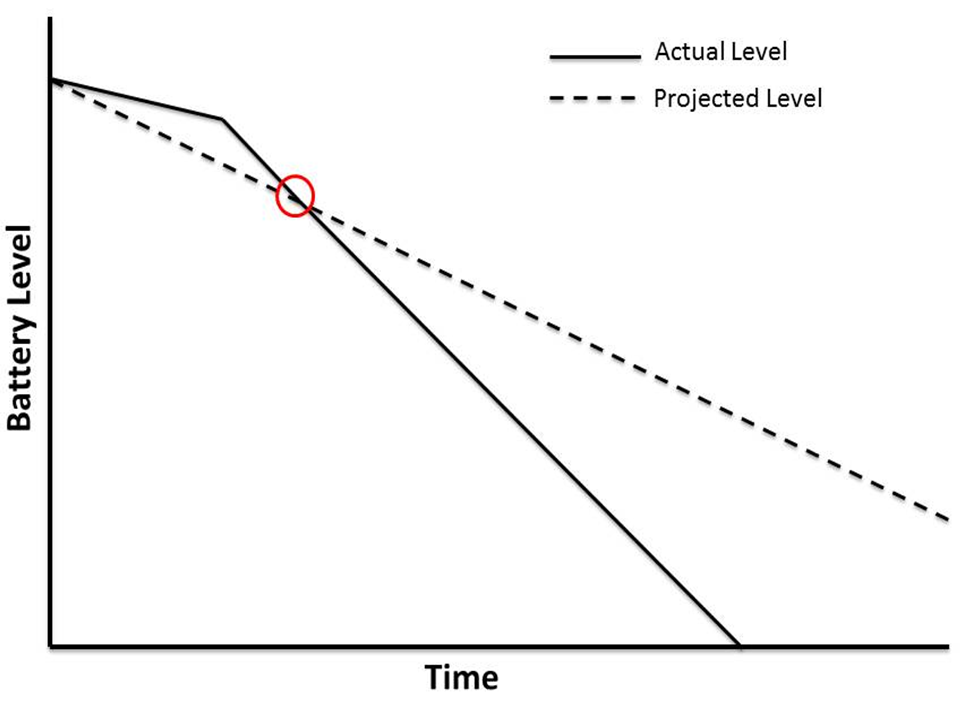
\includegraphics[width=\columnwidth]{figs/bat_vs_time.png}
		\caption{Battery level and projected level}
		\label{fig:bat_v_time}
\end{center}
\end{figure}
%%re-incorporate example?
% I like the example-- we should maybe provide it here or ? 
%   & not interspersed with implementation details
%   some sort of chart: time v. battery with prediction lines
% 
%Foremost, one must weigh the importance of recent data versus historic data.  
%A user's device usage rate is not likely to stay constant throughout the day.  
%For the majority of the day, the device might sit idle with occasional high power draining applications. 
%As a result, the long term usage rate alone cannot be the sole representation for analyzing and predicting the remaining time.  
%A common example would be a device that has been on idle for nearly a whole day.  
%The long term rate at this point would be a slow decrease that has left the phone low on remaining battery.  
%For the next five minutes, the user begins playing a CPU and network intensive game.  
%The user then wants to know if their device will last another hour.  
%If only the long term rate is used, that last five minute high usage rate is lost amongst the previous 24 hours.  
%However, the user is likely to continue running the game in the immediate future.  
%The long term collection and the most recent usage are combined with specific weights to create the most insightful recommendation possible. 
%With the overall rate and predicted end time determined, the application will be able to identify the primary culprits in the battery drain.  
%For our project, a culprit is an application that uses battery through intensive CPU or network use.  
%When the analyzer is started, Watt's Happening cycles through the list of currently running applications.  
%As stated in the assumptions section, only currently running applications are candidates for termination.  
%The analyzer considers the recent behavior as captured into the database and calculates the CPU and network use designated to each UID during the duration that it has been running.  
%With the CPU and network cost assigned to each culprit, the analyzer can determine the approximate cost of each culprit by combining those values with the amount of battery drained overall during the time period that the application was running.  
%The resulting value is used as a heuristic variable to allow comparisons between culprits and the follow-on recommendations to the user.
%\subsection*{Making Recommendations}
%The key to the success of Watt's Happening is arming the user with knowledge of their use and make knowledgeable recommendation to keep the device alive.  
%The logged information keep over a time period displaying the battery percentage versus time on a graph allows a graphical representation for the user to observe their usage habits. 
%The rate determined in the analyzer depicts on the graph the predicted battery termination time.  
%Should that time end before the user's goal, the application can display the top culprits currently running so the user is made aware of their candidates to close in order to reach their desired end time.
\subsection*{Display} %TODO why we display what we do how we do dododo
Upon request, \emph{Watt's Happening} displays to the user currently running applications sorted by resource consumption.
This allows the user to see at a glance which applications are impacting their battery use rate. %change this
The user can then view the estimate of time remaining and decide if any action, including terminating a running application, must be taken.
